\documentclass[11pt]{article}
\usepackage[margin=1in]{geometry}
\usepackage{amsmath,amssymb,amsthm}
\usepackage{hyperref}
\usepackage{booktabs}
\usepackage{tikz}
\usetikzlibrary{arrows.meta,positioning,fit,calc,shapes.geometric}

\newcommand{\R}{R_q}
\newcommand{\sample}{\mathrel{\leftarrow\joinrel\$}}
\newcommand{\roundp}[1]{\left\lceil #1\right\rfloor_p}

\newtheorem{theorem}{Theorem}[section]
\newtheorem{lemma}[theorem]{Lemma}

\title{Single-Key Cut-and-Choose for Keyed-Verification\\
Blind-Signature Credentials:\\A Compact Construction and its Security Intuition}
\author{}
\date{}
\begin{document}
\maketitle

\begin{abstract}
A blind signature lets a user obtain a credential without revealing its
message to the signer.  In the BLNS23 scheme, proving that the user's request
is well formed is expensive because the proof must check hash computations.
Replacing this proof with cut-and-choose run in parallel lanes avoids it
entirely.  This document explores a compact form of that idea: the signer
holds \emph{one} key, and the user commits to all branches at once by summing
them into a single aggregate, binding each branch individually by a hash.
The user sends the aggregate, the seeds of the branches selected for
checking, and the hashes of the unopened branches; the challenge is taken
over the aggregate and the full list of branch hashes, so the branch table is
fixed before the challenge exists.  The signer \emph{peels} the opened
branches off the aggregate and signs the remaining sum.  The first message
then carries one commitment vector, $\kappa$ seeds, and $\kappa$ hashes:
with the BLNS23 keyed-verification parameters and $\kappa=512$ lanes, about
$143$~KiB.  We give the construction, its correctness calculation, drawings
of the exchange, and a random-oracle analysis of its security core.  The
design's key property is \emph{structured-sum fixpoint hardness}: roughly,
that no attacker can force the signed sum into a chosen shape without about
$2^{\kappa/2}$ work.  We prove this property for the challenge game in the
classical random-oracle model (Theorem~\ref{thm:fixpoint}): an attacker
making $Q_h$ challenge-hash queries and completing $Q$ sessions aims a
peeled sum at a committed target set $T$, or places two accepted sessions in
a committed relation $T_{\mathrm{rel}}$, only with probability
$O\bigl(Q_h\,(|T|+Q\,|T_{\mathrm{rel}}|)\,2^{-\kappa}\bigr)$, and every
accepted session retains more than $\kappa/2$ honestly formed,
challenge-selected branch vectors except with probability
$Q_h\,2^{-\kappa/2}$.  The remaining lattice step is isolated as a single
decisional assumption, \emph{structured-sum HMLWE}
(Section~\ref{sec:latticestep}): key recovery reduces to it, linear
distinguishing strategies reduce to module-SIS or to the proven bounds,
residual control over the samples is priced by density, one-more
unforgeability follows from it together with the common-message binding, and
we explain why no reduction to plain MLWE can reach it.  The assumption
itself, its quantum analogue, and the simulation details of the one-more
hybrids remain open (Section~\ref{sec:proofneeds}).  Under that assumption
the best attacks we know are the copying-and-combining attacks of
Section~\ref{sec:splicing}, costing about $2^{\kappa/2}$ classical or
$2^{\kappa/4}$ quantum work, so $\kappa=512$ is the starting point.
\end{abstract}

\begin{center}
\fbox{\parbox{0.92\linewidth}{\textbf{Security status.}
The challenge-game core of the construction is proven in the classical
random-oracle model (Section~\ref{sec:romproof},
Theorem~\ref{thm:fixpoint}).  The remaining lattice step is isolated as one
decisional assumption, structured-sum HMLWE, with the surrounding links
proven: key recovery and one-more unforgeability reduce to it, and no
reduction from a standard assumption is available along known lines
(Section~\ref{sec:latticestep}).  The proof does not extend to quantum query
access, the isolated assumption is unproven, and the one-more simulation
details are uninstantiated (Section~\ref{sec:proofneeds}).
The scheme must not be deployed as a secure credential system.}}
\end{center}

\section{Introduction}

In the keyed-verification blind signature of Beullens, Lyubashevsky, Nguyen,
and Seiler (BLNS23)~\cite{BLNS23}, the user's first message contains a
zero-knowledge proof that a lattice commitment was formed correctly, including
correct evaluations of hash functions.  That proof dominates the cost of
issuance.

Cut-and-choose offers a different route: the user prepares many candidate
\emph{branches}, reveals some of them for checking, and the signer uses only
the unchecked rest.  Run in $\kappa$ parallel \emph{lanes}, in the spirit of
parallel-instance cut-and-choose~\cite{PCC22}, the idea replaces the
well-formedness proof with per-lane spot checks.  This document explores a
compact form of the construction:

\begin{itemize}
 \item \textbf{One key.}  The signer holds a single secret vector $\mathbf s$
and a single public matrix $B$.  There are no lane keys.
 \item \textbf{One aggregate commitment, bound leaf by leaf.}  The user sums
all $2\kappa$ branch vectors into a single aggregate $\mathbf
c_{\mathrm{agg}}$ and commits to each branch individually by a \emph{leaf
hash}.  The cut-and-choose challenge is derived from the aggregate together
with all $2\kappa$ leaf hashes, so the branch table is committed before the
challenge exists.  The individual branch vectors are never transmitted:
opened branches are regenerated from seeds, unopened branches are committed
by their hashes only.
 \item \textbf{Peeling.}  The signer recomputes the challenge, expands the
opened branches from their seeds, subtracts them from the aggregate, and signs
the remaining sum with its one key.
\end{itemize}

The appeal is concrete.  With the BLNS23 keyed-verification parameters and
$\kappa=512$ lanes, the first message carries a single commitment vector,
$\kappa$ seeds, and $\kappa$ leaf hashes: about $143$~KiB, none of it a proof
of hash evaluations.  The signer's response proof covers a single linear key
relation, and the signer stores one key.

The cost is equally concrete, and we state it up front: the BLNS23 proof
route --- extraction from the user's well-formedness proof --- no longer
exists, because cut-and-choose removed that proof, and the selected branches
are never revealed in any extractable form: their leaf hashes commit without
opening.  No replacement reduction is known, and
Section~\ref{sec:latticestep} explains why none can exist along known lines.
Security here rests on the interaction of the challenge hash with the
aggregate, which we call \emph{structured-sum fixpoint hardness}; we prove
its challenge-game content in the classical random-oracle model
(Section~\ref{sec:romproof}), and we isolate the step from its conclusion to
lattice hardness as a single decisional assumption, proving the links around
it (Section~\ref{sec:latticestep}).

\paragraph{Roadmap.}
Section~\ref{sec:notation} fixes notation.  Section~\ref{sec:construction}
gives the construction with drawings.  Section~\ref{sec:correctness} shows why
honest credentials verify.  Section~\ref{sec:intuition} gives the security
intuition and analysis: the commit-before-challenge order, the fixpoint wall,
the sum-to-target (Wagner) analysis, a random-oracle proof of the fixpoint
game, the isolation of the remaining lattice step, the splicing attacks and
their costs, the common-message strengthening that demotes splicing to
duplication, and blindness.  Section~\ref{sec:efficiency} estimates sizes.
Section~\ref{sec:proofneeds} lists what remains unproven.

\section{Notation and basic tools}
\label{sec:notation}

We work in the setting of the BLNS23 keyed-verification
instantiation~\cite{BLNS23}.  Let $\R$ be its ring, with
dimension $d=64$ and $\lceil\log_2 q\rceil=152$.  Vectors of $n=93$ ring
elements are written in bold, as are matrices.  The rounding map
$\roundp{\cdot}:\R\rightarrow R_p$ with $p=4$ keeps the high bits of each
coefficient.  A 32-byte seed $z$ is expanded by an extendable-output function
(XOF) into pseudorandom bytes; a fixed sampling procedure turns those bytes
into messages and bounded-distribution vectors.  Labels fed to hash functions
are distinct strings that separate the different uses.

A \emph{lane} is an index $i\in\{0,\ldots,\kappa-1\}$.  A \emph{branch} is one
of two candidates $b\in\{0,1\}$ prepared in a lane.  A \emph{session} is one
issuance attempt, identified by a session identifier $\mathsf{sid}$ that names
the protocol version, the issuer, and the key epoch, and carries fresh values
from both parties.

\section{The construction}
\label{sec:construction}

\subsection{Preparing the branches}

The user independently constructs two branches in each lane.  It samples a
32-byte seed $z_{i,b}$ and expands it:
\[
 (m_{i,b},\mathbf r_{i,b},\mathbf e_{2,i,b})
 =G(\mathsf{sid},i,b,z_{i,b}),
\]
where $m_{i,b}$ is 32 bytes and the two vectors have the prescribed bounded
distributions.  It computes
\begin{align*}
 \rho_{i,b}&=H_\rho(\mathsf{sid},i,b,
                     \mathbf r_{i,b},\mathbf e_{2,i,b}),\\
 \mathbf u_{i,b}&=H_R(\mathsf{credential\mbox{-}lane},i,m_{i,b},\rho_{i,b}),\\
 \mathbf c_{i,b}&=B\,\mathbf r_{i,b}+\mathbf e_{2,i,b}+\mathbf u_{i,b},\\
 \ell_{i,b}&=H_{\mathrm{leaf}}(\mathsf{sid},i,b,\mathbf c_{i,b}).
\end{align*}
Three details are essential later.  First, the tag $\rho_{i,b}$ binds the
branch to its session: valid branches can never be reused across sessions.
Second, the lane index $i$ sits \emph{inside} the lane hash $H_R$, so a branch
prepared for lane $i$ is meaningless in any other lane, even though all lanes
share the same matrix $B$.  Dropping the lane label would let an attacker move
branches between lanes freely; it is mandatory here.  Third, the \emph{leaf
hash} $\ell_{i,b}$ commits the branch to its position $(i,b)$ and to the
session before the challenge exists; because it covers $\mathsf{sid}$, even
content that is never opened cannot be replayed across sessions.
Section~\ref{sec:aggregate} explains why the challenge must be taken over
these leaves and over the aggregate alike.

\begin{figure}[t]
\centering
\resizebox{\linewidth}{!}{%
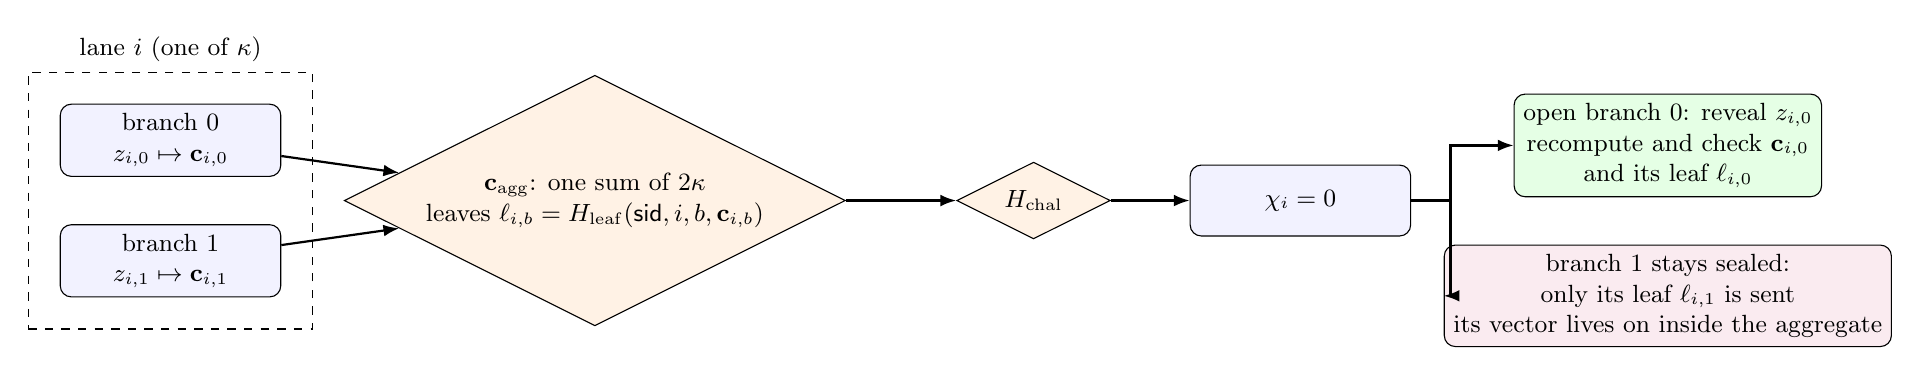
\begin{tikzpicture}[
  font=\small,
  node distance=6mm and 10mm,
  box/.style={draw,rounded corners,align=center,minimum height=9mm,
              minimum width=28mm,fill=blue!5},
  hash/.style={draw,diamond,aspect=2,align=center,fill=orange!10},
  ok/.style={draw,rounded corners,align=center,fill=green!10},
  keep/.style={draw,rounded corners,align=center,fill=purple!8},
  arrow/.style={-{Latex[length=2mm]},thick}
]
\node[box] (b0) {branch $0$\\$z_{i,0}\mapsto\mathbf c_{i,0}$};
\node[box,below=of b0] (b1) {branch $1$\\$z_{i,1}\mapsto\mathbf c_{i,1}$};
\node[hash,right=22mm of $(b0)!0.5!(b1)$] (sum) {$\mathbf c_{\mathrm{agg}}$:
 one sum of $2\kappa$\\ leaves $\ell_{i,b}=H_{\rm leaf}(\mathsf{sid},i,b,
 \mathbf c_{i,b})$};
\node[hash,right=14mm of sum] (chal) {$H_{\rm chal}$};
\node[box,right=of chal] (chi) {$\chi_i=0$};
\draw[arrow] (b0) -- (sum);
\draw[arrow] (b1) -- (sum);
\draw[arrow] (sum) -- (chal);
\draw[arrow] (chal) -- (chi);

\node[ok,right=13mm of chi,yshift=7mm] (open)
 {open branch $0$: reveal $z_{i,0}$\\recompute and check $\mathbf c_{i,0}$\\
  and its leaf $\ell_{i,0}$};
\node[keep,below=of open] (hidden)
 {branch $1$ stays sealed:\\only its leaf $\ell_{i,1}$ is sent\\its vector
  lives on inside the aggregate};
\draw[arrow] (chi.east) -- ++(5mm,0) |- (open.west);
\draw[arrow] (chi.east) -- ++(5mm,0) |- (hidden.west);
\node[draw,dashed,fit=(b0)(b1),inner sep=4mm,
      label={[font=\small]above:lane $i$ (one of $\kappa$)}] {};
\end{tikzpicture}%
}
\caption{One lane under the aggregate commitment.  Both branches enter the
single sum $\mathbf c_{\mathrm{agg}}$ and the leaf list; the challenge is
taken over both, so the branch table is fixed before $\boldsymbol\chi$
exists.  The challenge bit $\chi_i$ elects which branch is opened and
checked.  The other branch is never transmitted or checked: only its leaf
hash is sent, and its vector remains inside the aggregate.  Roles reverse
when $\chi_i=1$.}
\label{fig:lane}
\end{figure}

\subsection{One aggregate commitment and the challenge}
\label{sec:aggregate}

The user sums all $2\kappa$ branch vectors into one aggregate
\[
 \mathbf c_{\mathrm{agg}}=\sum_{i=0}^{\kappa-1}
 \bigl(\mathbf c_{i,0}+\mathbf c_{i,1}\bigr)\in\R^{n},
\]
and only then derives the challenge from the aggregate and the complete leaf
list
\[
 \boldsymbol\chi=(\chi_0,\ldots,\chi_{\kappa-1})
 =H_{\mathrm{chal}}(\mathsf{protocol},\mathsf{issuer},\mathsf{pk},
   \mathsf{sid},\mathbf c_{\mathrm{agg}},\
   \ell_{0,0},\ell_{0,1},\ldots,\ell_{\kappa-1,0},\ell_{\kappa-1,1})
   \in\{0,1\}^{\kappa}.
\]
Both inputs are load-bearing, for different reasons.  The leaf hashes fix the
branch \emph{table} --- which vector occupies each position $(i,b)$ ---
before the challenge exists.  Without them the challenge would commit only to
a sum, and a sum does not determine its summands: the user could choose the
decomposition of the aggregate into branches \emph{after} seeing the
challenge, and the per-lane soundness argument of Section~\ref{sec:hiding}
would not apply.  The aggregate must additionally enter the challenge itself,
because it is the value the signer peels: the leaves can never constrain it,
since the signer never learns the unopened preimages and consistency of the
aggregate with the table cannot be checked.  If the challenge did not cover
the aggregate, the user could fix the table, learn $\boldsymbol\chi$, and
only then choose the aggregate so that the peeled sum equals a chosen vector
--- the key-recovery attack of Section~\ref{sec:order} at constant cost.  The
encoding of the aggregate and the leaf list must be canonical and the domain
separation labels fixed, so that the hash input has only one interpretation.

The first message is
\[
 \mathsf{User}\longrightarrow\mathsf{Signer}:\quad
 \mathsf{sid},\ \mathbf c_{\mathrm{agg}},\
 \{z_{i,\chi_i}\}_{i=0}^{\kappa-1},\
 \{\ell_{i,\,1-\chi_i}\}_{i=0}^{\kappa-1}.
\]
Note what is \emph{not} sent: the unopened branch vectors.  The opened leaves
are recomputed from the seeds; the unopened leaves arrive as hashes only.
The aggregate remains the only commitment to the \emph{values}, but the leaf
list is a commitment to the \emph{table}: every branch, including junk that
is never opened, is position-bound and session-bound before the challenge
exists.

\subsection{Peeling and the aggregate response}
\label{sec:peeling}

The signer expands every revealed seed, reconstructs each opened branch, and
computes its leaf hash.  Together with the received unopened leaf hashes this
reassembles the full leaf list, and the signer recomputes $\boldsymbol\chi$
from the received aggregate and that list.  It checks that each reconstructed
branch was formed for this session and lane (labels, session identifier,
lattice equation, size bounds, encoding), and reconstructs the opened set
$\{\mathbf c_{i,\chi_i}\}_i$.  If any check fails it stops without returning
any secret-dependent value.  Otherwise it \emph{peels} the opened branches
off the aggregate:
\[
 \mathbf C_{\mathrm{sel}}
 =\mathbf c_{\mathrm{agg}}-\sum_{i=0}^{\kappa-1}\mathbf c_{i,\chi_i}
 =\sum_{i=0}^{\kappa-1}\mathbf c_{i,\,1-\chi_i}.
\]
We call $b_i^*=1-\chi_i$ the \emph{selected branch} in lane $i$ and write
$(m_i^*,\rho_i^*,\mathbf r_i^*,\mathbf e_{2,i}^*)$ for its contents.
The signer never sees the selected vectors individually; it holds only their
sum.

The signer derives a small deterministic error from its secret key $K$ and the
complete received input,
\[
 e=H_{D_e}(K,\mathsf{sid},\mathbf c_{\mathrm{agg}}),
\]
and answers with the aggregate response
\[
 h=\mathbf s^{T}\mathbf C_{\mathrm{sel}}+e\in\R,
\]
together with one zero-knowledge proof of the single-key response relation
\[
 \mathcal R_{\mathrm{resp}}:\quad
 \begin{cases}
  h=\mathbf s^{T}\mathbf C_{\mathrm{sel}}+e,\\
  \mathbf t^{T}=\mathbf s^{T}B+\mathbf e_{1}^{T},\\
  \|\mathbf s\|\leq\beta_s,\ \|\mathbf e_1\|\leq\beta_e,\ \|e\|\leq\beta_e.
 \end{cases}
\]
Because there is one key, the proof covers one key relation.  These are linear
lattice equations and norm bounds, provable with a LaBRADOR-style
proof~\cite{BS22}, and they avoid the hash evaluations that made the BLNS23
user proof expensive.  The signer releases only $h$ and the proof: partial
sums, per-lane values, failure details, and timing must not leak
secret-dependent information.

\begin{figure}[t]
\centering
\resizebox{\linewidth}{!}{%
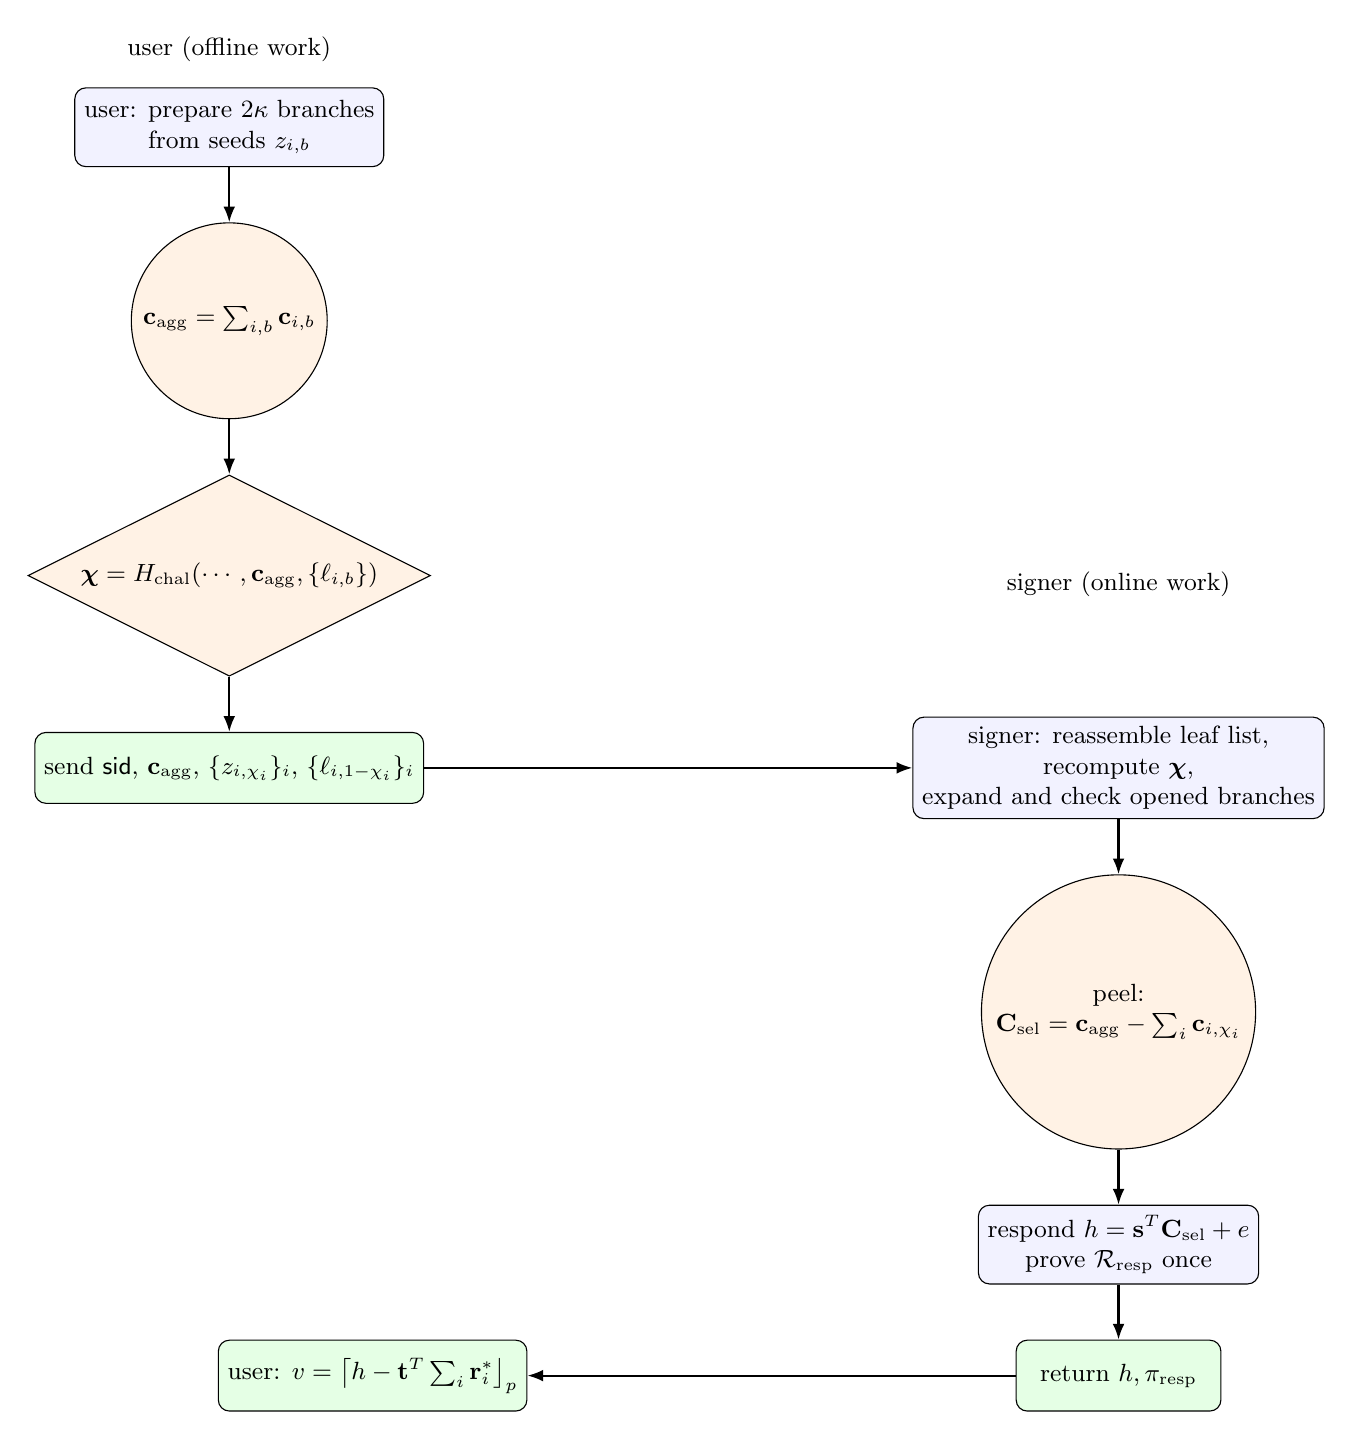
\begin{tikzpicture}[
  font=\small,
  node distance=7mm and 9mm,
  box/.style={draw,rounded corners,align=center,minimum height=10mm,
              minimum width=30mm,fill=blue!5},
  hash/.style={draw,diamond,aspect=2,align=center,fill=orange!10},
  op/.style={draw,circle,fill=orange!10,align=center,minimum size=10mm},
  result/.style={draw,rounded corners,align=center,fill=green!10,
                 minimum width=26mm,minimum height=9mm},
  arrow/.style={-{Latex[length=2mm]},thick}
]
% user column
\node[box] (prep) {user: prepare $2\kappa$ branches\\from seeds
 $z_{i,b}$};
\node[op,below=of prep] (agg) {$\mathbf c_{\mathrm{agg}}=\sum_{i,b}
 \mathbf c_{i,b}$};
\node[hash,below=of agg] (chal) {$\boldsymbol\chi=
 H_{\rm chal}(\cdots,\mathbf c_{\mathrm{agg}},\{\ell_{i,b}\})$};
\node[result,below=of chal] (send) {send $\mathsf{sid}$,
 $\mathbf c_{\mathrm{agg}}$, $\{z_{i,\chi_i}\}_i$,
 $\{\ell_{i,1-\chi_i}\}_i$};
\draw[arrow] (prep) -- (agg);
\draw[arrow] (agg) -- (chal);
\draw[arrow] (chal) -- (send);

% signer column
\node[box,right=62mm of send] (chk) {signer: reassemble leaf list,\\
 recompute $\boldsymbol\chi$,\\ expand and check opened branches};
\node[op,below=of chk] (peel) {peel:\\
 $\mathbf C_{\mathrm{sel}}=\mathbf c_{\mathrm{agg}}-\sum_i
 \mathbf c_{i,\chi_i}$};
\node[box,below=of peel] (resp) {respond
 $h=\mathbf s^{T}\mathbf C_{\mathrm{sel}}+e$\\
 prove $\mathcal R_{\rm resp}$ once};
\node[result,below=of resp] (ret) {return $h,\pi_{\rm resp}$};
\draw[arrow] (chk) -- (peel);
\draw[arrow] (peel) -- (resp);
\draw[arrow] (resp) -- (ret);

\draw[arrow] (send) -- (chk);

% user unblind
\node[result,left=62mm of ret] (unblind) {user:
 $v=\roundp{h-\mathbf t^{T}\sum_i \mathbf r_i^*}$};
\draw[arrow] (ret) -- (unblind);

\node[font=\small,above=2mm of prep] {user (offline work)};
\node[font=\small,above=14mm of chk] {signer (online work)};
\end{tikzpicture}%
}
\caption{The two-message exchange.  The user does all branch work offline and
sends one aggregate vector, $\kappa$ seeds, and $\kappa$ leaf hashes.  The
signer's online work is: reassemble the leaf list and recompute the
challenge, expand and check $\kappa$ opened branches, one subtraction per
opened branch, one inner product under its single key, and one single-key
proof.}
\label{fig:flow}
\end{figure}

\subsection{Finishing and presenting the credential}

After checking the response proof, the user removes the blinding terms one
branch at a time and rounds:
\[
 v=\roundp{h-\mathbf t^{T}\sum_{i=0}^{\kappa-1}\mathbf r_i^*},
 \qquad
 \sigma=\bigl((m_i^*,\rho_i^*)_{i=0}^{\kappa-1},\,v\bigr).
\]
The selected seeds stay private even at presentation: a seed would reveal the
blinding vectors and let the issuer match the credential to its issuance.

At presentation, the verifier (which holds the same key) recomputes the
expected value and accepts exactly when
\[
 v=\roundp{\mathbf s^{T}\sum_{i=0}^{\kappa-1}
        H_R(\mathsf{credential\mbox{-}lane},i,m_i^*,\rho_i^*)}.
\]
The lane hash used at presentation must not
contain the issuance session identifier; the session identifier is bound into
branch formation and the challenge only.  An application derives one payload
from the ordered message/tag list:
\[
 M=H_{\mathrm{final}}(\mathsf{issuer},\mathsf{type},
              (m_i^*,\rho_i^*)_{i=0}^{\kappa-1}).
\]

\section{Why honest credentials verify}
\label{sec:correctness}

The unblinding step cancels most of the noise.  For an honestly generated
selected branch,
\[
 \mathbf s^{T}\mathbf c_i^*-\mathbf t^{T}\mathbf r_i^*
 =\mathbf s^{T}\mathbf u_i^*
  +\bigl(\mathbf s^{T}\mathbf e_{2,i}^*-\mathbf e_1^{T}\mathbf r_i^*\bigr),
\]
so
\[
 h-\mathbf t^{T}\sum_i\mathbf r_i^*
 =\mathbf s^{T}\sum_i\mathbf u_i^*
  +\underbrace{\sum_i\bigl(\mathbf s^{T}\mathbf e_{2,i}^*
       -\mathbf e_1^{T}\mathbf r_i^*\bigr)+e}_{\text{correctness error}}.
\]
The verifier recomputes the main term from the presented messages and tags.
Acceptance requires that the correctness error never crosses a rounding
boundary.  The per-branch error terms have the same shape as in BLNS23's own
verification equation, but here they are summed over $\kappa$ lanes: the
error is a sum of $2\kappa+1$ small terms, so its size grows
with the lane count (about $\sqrt{\kappa}$ in the typical randomized model,
$\kappa$ in the worst case), and all terms
share one secret $\mathbf s$ and one public-key error $\mathbf e_1$.

\section{Security analysis}
\label{sec:intuition}

We state the attacks we know, the design rules they force, the part of the
security claim that can be proven in the random-oracle model
(Section~\ref{sec:romproof}), and the isolation of the part that cannot
(Section~\ref{sec:latticestep}).

\subsection{The load-bearing order: commit before challenge}
\label{sec:order}

The aggregate and the branch table must be fixed before the challenge exists.
To see why, suppose for a moment the opposite: the user learns
$\boldsymbol\chi$ (or its effect on which branches are opened) before fixing
$\mathbf c_{\mathrm{agg}}$.  Then the user can pad the aggregate with a junk
term
\[
 J=\mathbf w-\sum_i \mathbf c_{i,\,1-\chi_i}
\]
so that the peeled value equals a \emph{chosen} vector $\mathbf w$.  Two
immediate consequences:

\begin{itemize}
 \item \textbf{Key recovery.}  With $\mathbf w$ the $j$-th unit vector, the
response is $h=s_j+e$: one secret-key coordinate plus small noise.  A handful
of sessions per coordinate, with fresh session identifiers decorrelating the
noise, recovers the entire secret key.
 \item \textbf{Free splicing.}  With $\mathbf w$ chosen to cancel the honest
content of a previous session and inject copied content, the copying attacks
of Section~\ref{sec:splicing} cost a constant number of hash trials instead of
an exponential search.
\end{itemize}

The construction forbids this by deriving $\boldsymbol\chi$ from the full
aggregate and the complete leaf list with a hash function modeled as a random
oracle, and by including fresh signer randomness in $\mathsf{sid}$.  The leaf
list is not optional here: if the challenge covered the leaves but not the
aggregate, the aggregate itself could be chosen after $\boldsymbol\chi$ is
known, and the same padding attack would return at constant cost
(Section~\ref{sec:aggregate}).  In a two-message protocol the
signer's fresh value must come from an authenticated session setup or a
previously established context; without it, the user can precompute entire
exchanges long before contact.  The order carries decisive weight here,
because it is the \emph{only} barrier: with a single key, nothing algebraic
separates one lane's vectors from another's (Section~\ref{sec:givesup}).

\subsection{Hiding malformed branches}
\label{sec:hiding}

Call a branch \emph{openable} if a seed regenerates it and it passes every
formation check.  The signer checks only opened branches, so an attacker that
wants a malformed branch to affect the response must keep it unopened.
Because the challenge covers the complete leaf list, the branch table is
fixed before the challenge exists: for a committed table containing one
openable and one malformed branch in each of $k$ attacked lanes, a uniform
challenge opens all $k$ openable branches with probability $2^{-k}$; each
Fiat--Shamir trial re-randomizes the challenge, so $q$ trials succeed with
probability at most about $q\,2^{-k}$.  Lemma~\ref{lem:sound} in
Section~\ref{sec:romproof} is the exact form of this bound.

The leaf binding is what makes this argument valid, and it repairs a real
defect of the bare aggregate.  A sum does not determine its summands: if the
challenge were taken over $\mathbf c_{\mathrm{agg}}$ alone, no branch table
would be committed at all, and the attacker could choose the decomposition of
the aggregate into branches \emph{after} computing the challenge ---
presenting whichever precomputed openable branches suit the realized
$\boldsymbol\chi$ and treating everything else as junk.  The probability
experiment above would then be the wrong one: per hash query the attacker
would succeed whenever \emph{any} favorable decomposition exists, a strictly
larger event whose analysis resembles a list-decoding problem rather than
$\kappa$ independent coin flips.  The leaf hashes eliminate this freedom at a
cost of $16$~KiB, and because each leaf covers $\mathsf{sid}$, even
never-opened junk is session-bound and cannot be replayed across sessions.

The essential point stands: an attacker may place
\emph{arbitrary} junk in unopened positions --- the peeled sum is never
checked --- but any junk must now be committed, per position and per session,
before the challenge is known, and the challenge decides which honest
branches remain in the sum.  The next subsection explains why this makes the
junk hard to aim.

\subsection{Why chosen inputs seem out of reach: the fixpoint wall}
\label{sec:fixpoint}

The dangerous attacks above all need the peeled sum $\mathbf C_{\mathrm{sel}}$
to land in a chosen shape: a unit vector for key recovery, or a previous
session's content for cancellation.  The attacker controls the aggregate, so
why can it not simply choose $\mathbf C_{\mathrm{sel}}$?

Because the honest branches it is forced to include interfere in a
challenge-dependent way.  Every lane must contain at least one openable branch
(otherwise the session is rejected with probability one), and the openable
branches are honestly formed, session-bound vectors whose values are fixed
once the leaf list is fixed.  The peeled sum is
\[
 \mathbf C_{\mathrm{sel}}
 =\underbrace{\sum_{i\in H}\mathbf c_{i,\,1-\chi_i}}_{\text{honest, chosen
    by }\boldsymbol\chi}
 \;+\;\underbrace{\sum_{i\in H^{c}}\mathbf w_i}_{\text{junk, committed
    before }\boldsymbol\chi},
\]
where $H$ is the set of lanes whose selected branch is honest.  To aim the
sum, the attacker must choose the junk to cancel the honest part --- but the
honest part is a pseudorandom function of the challenge, and the challenge is
a pseudorandom function of the aggregate, the junk included.  The dependency
is circular:
choosing $J$ fixes $\mathbf c_{\mathrm{agg}}$, which fixes
$\boldsymbol\chi$, which fixes the honest selected sum, which determines the
$J$ that would have been needed (Figure~\ref{fig:fixpoint}).

\begin{figure}[t]
\centering
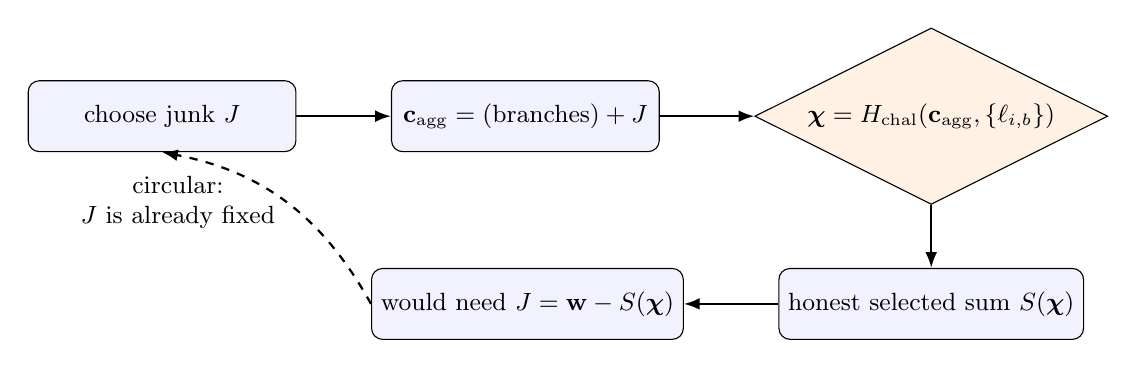
\begin{tikzpicture}[
  font=\small,
  node distance=8mm and 12mm,
  box/.style={draw,rounded corners,align=center,minimum height=9mm,
              minimum width=34mm,fill=blue!5},
  hash/.style={draw,diamond,aspect=2,align=center,fill=orange!10},
  arrow/.style={-{Latex[length=2mm]},thick}
]
\node[box] (J) {choose junk $J$};
\node[box,right=of J] (cagg) {$\mathbf c_{\mathrm{agg}}=
 (\text{branches})+J$};
\node[hash,right=of cagg] (X) {$\boldsymbol\chi=
 H_{\rm chal}(\mathbf c_{\mathrm{agg}},\{\ell_{i,b}\})$};
\node[box,below=of X] (S) {honest selected sum $S(\boldsymbol\chi)$};
\node[box,left=of S] (need) {would need $J=\mathbf w-S(\boldsymbol\chi)$};
\draw[arrow] (J) -- (cagg);
\draw[arrow] (cagg) -- (X);
\draw[arrow] (X) -- (S);
\draw[arrow] (S) -- (need);
\draw[arrow,dashed] (need.west) to[bend right=25]
 node[midway,left,align=center]{circular:\\$J$ is already fixed} (J.south);
\end{tikzpicture}
\caption{The fixpoint wall.  Aiming the peeled sum at a target $\mathbf w$
requires junk that cancels a challenge-dependent honest sum; the junk is
committed before the challenge exists.  Resolving the cycle is a search:
guess the challenge pattern, set the junk accordingly, and hope the hash
returns the guessed pattern.}
\label{fig:fixpoint}
\end{figure}

Resolving the cycle is a guess-and-check search.  Guessing the full challenge
pattern costs about $2^{\kappa}$ trials (or $2^{\kappa/2}$ with generic
quantum search).  A meet-in-the-middle variant that only asks for a chosen
\emph{difference} between two sessions' peeled sums --- enough for the
key-recovery attack --- costs about $2^{\kappa/2}$ classical trials.
We know no cheaper route.  This motivates the property on which everything
here rests, stated informally here and proven for the challenge game in
Section~\ref{sec:romproof}:

\begin{center}
\fbox{\parbox{0.92\linewidth}{\textbf{Structured-sum fixpoint hardness
(informal statement; formal version and proof in
Section~\ref{sec:romproof}).}  Consider an attacker that may prepare branch
tables freely, make $q$ random-oracle queries, and run $Q$ issuance sessions
against the construction of Section~\ref{sec:construction}.  Then, except
with probability on the order of $q\,2^{-\kappa/2}$, every accepted session's
peeled sum $\mathbf C_{\mathrm{sel}}$ is \emph{uncontrolled}: its honest
content is a set of honestly formed, session-fresh, hash-derived branch
vectors whose selection is decided by the challenge only after the table is
committed, and no two accepted sessions' peeled sums satisfy a linear
relation committed before the later session's challenge query.}}
\end{center}

Given this property, the responses $h=\mathbf s^{T}\mathbf
C_{\mathrm{sel}}+e$ are learning-with-errors samples whose public vectors the
attacker can influence but not aim.  Whether such samples are safe --- and
what exactly must be assumed to conclude that they are --- is the subject of
Section~\ref{sec:latticestep}, which isolates the step as one decisional
assumption (structured-sum HMLWE) and proves the links around it.

\subsection{Why not a sum-to-target attack?}
\label{sec:wagner}

The most direct attempt on the fixpoint wall treats the aggregate as a sum to
be solved: grind seeds to build a list of candidate vectors at every
position, then search for a table whose unopened branches sum to a chosen
target,
\[
 \sum_{i=0}^{\kappa-1} \mathbf c_{i,\,1-\chi_i}=\mathbf w,
 \qquad
 \boldsymbol\chi=H_{\mathrm{chal}}(\mathsf{sid},\mathbf
   c_{\mathrm{agg}},\{\ell_{i,b}\}),
\]
or equivalently choose $\mathbf c_{\mathrm{agg}}$ adversarially and search
for opened branches summing to $\mathbf c_{\mathrm{agg}}-\mathbf w$.  Two
constraints stack, and each repays careful reading.

\paragraph{The vector equality is exact, and the space is enormous.}
Exactness is forced: key recovery needs $\mathbf C_{\mathrm{sel}}$ to isolate
key coordinates, splicing needs previous sessions' lane values reproduced
exactly because the presentation check is over exact hash images, and an
approximate hit $\mathbf w+\boldsymbol\delta$ does not isolate anything,
since $\mathbf s^{T}\boldsymbol\delta$ is secret-dependent.  The target is
therefore one value in a space of bit-length
$N=n\,d\,\lceil\log_2 q\rceil=93\cdot64\cdot152\approx 904{,}704$ bits.
Sum-to-target over per-lane lists is the generalized birthday problem, solved
by Wagner's $k$-tree algorithm~\cite{Wag02} --- and its cost scales with the
bit-length of the sum space, not with the security parameter: with $\kappa$
lists it uses time and list size about
$2^{N/(1+\lfloor\log_2\kappa\rfloor)}$.  At $\kappa=512$ this is about
$2^{90{,}470}$: the per-lane lists alone would require grinding that many
seeds per lane.  Even the information-theoretic minimum for a solution to
exist is $\kappa\,t\ge N$ for lists of size $2^t$, i.e.\ $t\approx1{,}767$
bits of seed grinding per position.  Exact aiming is not a $128$-bit problem
but a $90{,}000$-bit one; the size of the ring --- the very thing that makes
the commitment vectors $113$~KiB each --- is what protects the construction.
And the challenge constraint stacks on top: a table that solved the sum would
still need $\boldsymbol\chi$ to select the intended complement.

\paragraph{Why the working attacks look different.}
The balanced splice (Section~\ref{sec:splicing}) and the meet-in-the-middle
difference attack described above never aim at a prescribed target: they
manufacture their targets from copied content, and committing a junk pair
with a chosen per-lane difference costs nothing.  The $N$-bit constraint
never bites; only the challenge-hiding cost remains, $2^{\kappa/2}$ classical
or $2^{\kappa/4}$ quantum.  The fixpoint property is, at heart, the claim
that no middle path exists --- no relaxation of exact aiming that stays
useful to the attacker yet becomes feasible.

\paragraph{Caveats.}
Two qualifications keep this honest.  First, relaxations: if a \emph{set} $T$
of dangerous peeled sums is exploitable --- say, all sufficiently sparse
differences rather than only unit vectors --- the effective attack cost
divides by $|T|$, and list-merging is exactly how an attacker would harvest
relaxed targets.  Bounding $|T|$ rigorously is priced by
Lemma~\ref{lem:grind}: every bit of $\log_2|T|$ comes directly off the
margin.  Second, the argument is parametric: it rests on
$N\gg\kappa\,(1+\log_2\kappa)$.  Shrinking the ring, the vector length, or
the challenge length to save bandwidth moves the construction toward the
regime where $2^{N/(1+\log_2\kappa)}$ crosses below $2^{\kappa/2}$ and
sum-to-target attacks become the cheapest ones.

\subsection{A random-oracle proof of the fixpoint game}
\label{sec:romproof}

We now prove the precise content of the boxed statement for the challenge
game, in the classical random-oracle model.  The proof covers everything the
challenge hash is responsible for --- hiding, aiming, and committed relations
between sessions.  What it does not cover is stated at the end.

\paragraph{The game.}
Model $G$, $H_\rho$, $H_R$, $H_{\mathrm{leaf}}$, and $H_{\mathrm{chal}}$ as
independent random oracles, and assume the signer never repeats a session
identifier.  Call a vector $\mathbf c\in\R^{n}$ \emph{openable at}
$(\mathsf{sid},i,b)$ relative to the attacker's query transcript if the
transcript contains the full chain: a seed $z$ with
$G(\mathsf{sid},i,b,z)=(m,\mathbf r,\mathbf e_2)$ inside the norm bounds,
the tag $\rho=H_\rho(\mathsf{sid},i,b,\mathbf r,\mathbf e_2)$, the image
$\mathbf u=H_R(\mathsf{credential\mbox{-}lane},i,m,\rho)$, and the equation
$\mathbf c=B\mathbf r+\mathbf e_2+\mathbf u$.  A \emph{committed input} is a
tuple $X=(\mathsf{sid},\mathbf c_{\mathrm{agg}},\ell_{0,0},\ell_{0,1},
\ldots,\ell_{\kappa-1,0},\ell_{\kappa-1,1})$; write
$\boldsymbol\chi(X)=H_{\mathrm{chal}}(\cdots,X)$.  For each position $(i,b)$
the attacker either knows a preimage $\mathbf c_{i,b}$ with
$H_{\mathrm{leaf}}(\mathsf{sid},i,b,\mathbf c_{i,b})=\ell_{i,b}$ or it does
not; a position is \emph{open} if a preimage is known and openable at
$(\mathsf{sid},i,b)$.  A lane is \emph{free} if both positions are open,
\emph{risky} if exactly one is, and \emph{dead} if neither is.  The session
is accepted exactly when the challenge position $\chi_i$ is open in every
lane and the attacker produces the corresponding seeds; the peeled sum is
then
\[
 \mathbf C_{\mathrm{sel}}(X,\boldsymbol\chi)
 =\mathbf c_{\mathrm{agg}}-\sum_{i=0}^{\kappa-1}\mathbf c_{i,\chi_i},
\]
well defined for acceptable $\boldsymbol\chi$ because the opened preimages
are openable, hence unique up to random-oracle collision.

Two features of the model do all the work.  First, $\boldsymbol\chi(X)$ is
uniform in $\{0,1\}^{\kappa}$ and independent of everything the attacker has
seen before the query at $X$; a session submitted without such a query is
answered at signing time and is counted as a query.  Second, the number of
committed inputs and openable chains the attacker can produce is bounded by
its query count.  Write $Q_h$ for the number of challenge-oracle queries
(including submitted sessions), $Q$ for the number of accepted sessions, and
$Q_R$ for the total number of random-oracle queries.

We condition throughout on two global events whose failure probabilities are
negligible at the parameters of Section~\ref{sec:efficiency}:
(i) \emph{oracle regularity}: no collisions occur in any random oracle, and
no openable chain exists that the attacker did not query --- failure
probability $O(Q_R^{2}\,2^{-256})$;
(ii) \emph{distinctness}: within each committed input, the values
$\mathbf C_{\mathrm{sel}}(X,\boldsymbol\chi)$ over acceptable
$\boldsymbol\chi$ are distinct.  A collision is an equation
$\sum_{i\in S}\pm(\mathbf u_{i,0}-\mathbf u_{i,1})=(\text{lattice parts})$
in the $H_R$ outputs for some nonempty $S\subseteq\{0,\ldots,\kappa-1\}$;
a union bound over committed inputs, subsets $S$, and tuples of $H_R$ queries
gives failure probability at most
$2^{\kappa}\,Q_R^{\,2\kappa+1}\,2^{-N}$ with
$N=n\,d\,\lceil\log_2 q\rceil\approx904{,}704$, which is negligible for any
$Q_R\ll 2^{N/(2\kappa)}\approx 2^{883}$.

\begin{lemma}[commit-then-challenge soundness]
\label{lem:sound}
For a committed input with $r$ risky lanes and no dead lane, the session is
accepted with probability $2^{-r}$ over $\boldsymbol\chi$; a dead lane makes
acceptance impossible.  Consequently
\[
 \Pr\bigl[\text{some accepted session has fewer than }\kappa/2
 \text{ free lanes}\bigr]\;\le\;Q_h\,2^{-\kappa/2}.
\]
\end{lemma}

\begin{proof}
Acceptance requires $\chi_i$ to name an open position in every lane, and
under the uniform $\boldsymbol\chi$ the lanes are independent: free lanes
always accept, risky lanes accept with probability $1/2$, dead lanes never.
The first claim follows.  An accepted session with fewer than $\kappa/2$ free
lanes has at least $\kappa/2$ risky lanes, so per committed input the
probability is at most $2^{-\kappa/2}$; the bound is a union over the at most
$Q_h$ committed inputs.
\end{proof}

Lemma~\ref{lem:sound} is the quantitative form of
Section~\ref{sec:hiding}.  Its content for what follows: outside a
$Q_h\,2^{-\kappa/2}$ exception, every accepted session has more than
$\kappa/2$ free lanes, and its peeled sum can be written in the affine form
\[
 \mathbf C_{\mathrm{sel}}(X,\boldsymbol\chi)
 =\mathbf C_0(X)+\sum_{i\in F}\chi_i\,\boldsymbol\Delta_i,
 \qquad
 \boldsymbol\Delta_i=\mathbf c_{i,0}-\mathbf c_{i,1},
\]
where $F$ is the free-lane set, $|F|>\kappa/2$, and every $\mathbf c_{i,b}$
is openable --- honestly formed and bound to $(\mathsf{sid},i,b)$.  At commit
time $\boldsymbol\chi$ is uniform and unknown, so the peeled sum is an
affine image of the challenge over more than $\kappa/2$ committed honest
differences.  This is the precise form of ``uncontrolled'': the attacker
learns $\boldsymbol\chi$ immediately after its query, so unpredictability
holds only at commit time, and changing the selection requires a new query.

\begin{lemma}[target avoidance]
\label{lem:target}
Fix a committed input $X$ and a target set $T\subseteq\R^{n}$, both chosen
before the challenge query at $X$ (they may depend arbitrarily on the
attacker's transcript so far).  Then, under distinctness,
\[
 \Pr_{\boldsymbol\chi}\bigl[\text{accepted}\ \wedge\
 \mathbf C_{\mathrm{sel}}(X,\boldsymbol\chi)\in T\bigr]
 \;\le\;|T|\,2^{-\kappa}.
\]
\end{lemma}

\begin{proof}
Acceptance is possible for at most $2^{|F|}$ challenge patterns, and by
distinctness the map
$\boldsymbol\chi\mapsto\mathbf C_{\mathrm{sel}}(X,\boldsymbol\chi)$ is
injective on them, so at most $|T|$ acceptable patterns land in $T$.  The
challenge is uniform over $2^{\kappa}$ patterns.
\end{proof}

For key recovery, $T$ is the set of peeled sums from which key material is
extractable --- unit vectors, and whatever sparse or structured vectors
suffice --- and the lemma prices the attack at
$Q_h\,|T|\,2^{-\kappa}$.  Every bit of $\log_2|T|$ comes directly off the
margin; Lemma~\ref{lem:grind} below extends the same pricing to target sets
the attacker does not commit but selects by rejection.

\begin{lemma}[committed-relation resistance]
\label{lem:relation}
Let session $1$ be accepted with peeled sum $\mathbf C_1$.  For any later
committed input $X_2$ and any relation set $T_{\mathrm{rel}}\subseteq\R^{n}$
committed together with $X_2$ --- after session $1$ completes, but before the
challenge query at $X_2$ --- the probability that $X_2$ is accepted and
$\mathbf C_2-\mathbf C_1\in T_{\mathrm{rel}}$ is at most
$|T_{\mathrm{rel}}|\,2^{-\kappa}$ under distinctness.  Union over inputs and
prior sessions: at most $Q_h\,Q\,|T_{\mathrm{rel}}|\,2^{-\kappa}$.
\end{lemma}

\begin{proof}
Identical to Lemma~\ref{lem:target} with
$T=\mathbf C_1-T_{\mathrm{rel}}$: at most $|T_{\mathrm{rel}}|$ acceptable
patterns for $\boldsymbol\chi(X_2)$ satisfy the relation, and
$\boldsymbol\chi(X_2)$ is uniform and independent of the attacker's view at
commit time, session $1$ included.
\end{proof}

\begin{theorem}[structured-sum fixpoint hardness, classical ROM]
\label{thm:fixpoint}
Let the signer enforce session-identifier uniqueness, and let
$|T|$ and $|T_{\mathrm{rel}}|$ be the largest target and relation sets the
attacker commits.  Then, except with probability
\[
 Q_h\,2^{-\kappa/2}
 \;+\;Q_h\,|T|\,2^{-\kappa}
 \;+\;Q_h\,Q\,|T_{\mathrm{rel}}|\,2^{-\kappa}
 \;+\;2^{\kappa}\,Q_R^{\,2\kappa+1}\,2^{-N}
 \;+\;O(Q_R^{2}\,2^{-256})
\]
over the random oracles, every session the attacker completes satisfies:
(i) its table has more than $\kappa/2$ free lanes, so its peeled sum is an
affine image of the challenge over more than $\kappa/2$ honestly formed,
session-fresh, hash-derived branch differences committed before the challenge
existed;
(ii) its peeled sum avoids every target set committed before the challenge
query;
(iii) its peeled sum stands in no committed relation to the peeled sum of any
previously accepted session.
\end{theorem}

\begin{proof}
Union bound over Lemmas~\ref{lem:sound}--\ref{lem:relation} and the two
conditioning events.
\end{proof}

\paragraph{Tightness.}
The bounds are matched by the attacks of the preceding subsections.  Hiding
$k$ malformed branches costs $2^{k}$ trials (Lemma~\ref{lem:sound}).  Aiming
at a fixed target with $|T|\approx1$ costs $2^{\kappa}$
(Lemma~\ref{lem:target}).  A committed difference between two sessions costs
$Q_h\,Q\,2^{-\kappa}\approx1$ at $Q_h\approx Q\approx2^{\kappa/2}$
(Lemma~\ref{lem:relation}) --- exactly the meet-in-the-middle and balanced
splice figures.  The $2^{\kappa/2}$ floor is therefore not an artifact of
missing analysis: it is where the proven bounds stop protecting the
construction.

\paragraph{What is not covered.}
Three things.  First, quantum query access: the proofs sample
$\boldsymbol\chi$ classically at query time and take union bounds over
classical query transcripts; a quantum attacker queries in superposition, and
the analysis needs compressed-oracle or equivalent techniques.  The
$2^{\kappa/4}$ quantum floor of Section~\ref{sec:splicing} is only a
generic-search estimate.  Second, the step from uncontrolled peeled sums to
lattice hardness: Theorem~\ref{thm:fixpoint} says the attacker cannot aim
$\mathbf C_{\mathrm{sel}}$, not that
$h=\mathbf s^{T}\mathbf C_{\mathrm{sel}}+e$ with uncontrolled
$\mathbf C_{\mathrm{sel}}$ is safe.  That step is taken up in
Section~\ref{sec:latticestep}, which isolates it as a single decisional
assumption (structured-sum HMLWE), proves the links from it to key recovery
and one-more unforgeability, and shows why no reduction to plain MLWE
applies; the assumption itself remains open.  Third, the simulation details
of the one-more accounting: the counting argument is
Theorem~\ref{thm:onemore}, but its hybrid steps --- response-proof
simulation, key validation, correctness --- remain uninstantiated.

\subsection{The lattice step: isolating the remaining assumption}
\label{sec:latticestep}

Theorem~\ref{thm:fixpoint} leaves a precise gap, and this subsection
determines exactly what fills it.  Condition on its good event.  Every
accepted session hands the attacker a sample
\[
 \bigl(\mathbf C_{\mathrm{sel}},\;h=\mathbf s^{T}\mathbf
 C_{\mathrm{sel}}+e\bigr),
 \qquad
 \mathbf C_{\mathrm{sel}}
 =\mathbf C_0(X)+\sum_{i\in F}\chi_i\,\boldsymbol\Delta_i,
 \qquad |F|>\kappa/2,
\]
in which \emph{every} vector on the right-hand side is known to the
attacker: it built the branch table, junk included.  The only quantity fixed
after commitment is the challenge, uniform over at least $|F|$ effective
bits of selection.  Issuance is therefore an oracle for
learning-with-errors samples whose matrices the attacker knows completely
and influences in exactly two ways: it chooses the table, and it chooses
which challenge queries to carry to completion.  The \emph{lattice step} is
the claim that such samples neither reveal $\mathbf s$ nor can be produced
without it.  We isolate that claim as one decisional assumption, prove the
links from it to key-recovery resistance and one-more unforgeability, price
the residual control the attacker retains over the matrices, and explain why
no reduction to a standard assumption is available along known lines.

\paragraph{Why no standard reduction applies.}
A reduction must answer issuance queries without knowing $\mathbf s$.  Both
classical routes die on the construction's two defining features.  First,
the single key: with independent lane keys, the reduction embeds its
challenge in one lane's key and computes the other lanes' contributions
locally, absorbing arbitrary content there; here every term of $\mathbf
C_{\mathrm{sel}}$ lives under the unknown $\mathbf s$, and no known-key lane
exists to absorb anything.  Second, the peeled sum is not a hash image: an
HMLWE-style oracle (as in BLNS23's Lemma~4.3) evaluates $\mathbf s$ only at
fresh outputs of $H_R$, but $\mathbf C_{\mathrm{sel}}$ contains committed
junk $\mathbf w$ that never passed through $H_R$.  Extraction is not the
obstacle --- the reduction can recover $\mathbf w$ from the attacker's
$H_{\mathrm{leaf}}$ query history --- but no oracle will supply $\mathbf
s^{T}\mathbf w$.  Knowing the key forfeits the embedded challenge; not
knowing it forfeits the junk term.  Repairing either route means arranging
for every term of the peeled sum to be a certified hash image, that is,
proving well-formedness of the unopened branches --- the very proof
cut-and-choose exists to eliminate.  The remaining assumption must therefore
be made explicit.

\begin{center}
\fbox{\parbox{0.92\linewidth}{\textbf{Structured-sum HMLWE (ssHMLWE).}
In the model of Section~\ref{sec:romproof}, an attacker plays the issuance
game of Section~\ref{sec:construction} against a challenger holding the
signer key, with session-identifier uniqueness enforced.  In the \emph{real}
game, each accepted session is answered by
$h=\mathbf s^{T}\mathbf C_{\mathrm{sel}}+e$; in the \emph{ideal} game, each
accepted session is answered by an independent uniform $h\sample\R$.
The assumption: every classical attacker making polynomially many queries
distinguishes the two games with advantage negligible beyond the error terms
of Theorem~\ref{thm:fixpoint}.}}
\end{center}

Three remarks delimit the assumption.  First, it is purely decisional: it
asserts pseudorandomness of the response stream and says nothing about
forgery by itself.  Second, the error terms are load-bearing, and they are
exactly the right ones: grinding two sessions to \emph{equal} peeled sums
would distinguish the games (then $h_1-h_2=e_1-e_2$ is small), and
Lemma~\ref{lem:target} with $|T|=1$ prices that at $2^{-\kappa}$ per query
pair; the known attacks at the $2^{\kappa/2}$ frontier are forgeries and
meet-in-the-middle searches, not distinguishers.  No attack on ssHMLWE
itself is known at any budget.  Third, the assumption is falsifiable in a
precise sense made explicit after Lemma~\ref{lem:grind} below.

\paragraph{Key recovery reduces to the assumption.}
The first link needs no lattice machinery at all, because a candidate key
can be checked against the attacker's own transcript.

\begin{theorem}[keys are self-verifying]
\label{thm:selfverify}
Let $\mathcal A$ be an attacker in the real issuance game that outputs the
signer key with probability $\delta$.  Then there is an ssHMLWE distinguisher
with advantage at least
\[
 \delta-\Bigl(\frac{2\beta_e+1}{q}\Bigr)^{d},
\]
where $\beta_e$ is the response-error bound of Section~\ref{sec:peeling}.
\end{theorem}

\begin{proof}
The distinguisher relays $\mathcal A$'s issuance sessions to its own
challenger and reads every $\mathbf C_{\mathrm{sel}}$ off the transcript.
When $\mathcal A$ outputs a candidate $\hat{\mathbf s}$, the distinguisher
guesses ``real'' if and only if
$\|h_j-\hat{\mathbf s}^{T}\mathbf C_{\mathrm{sel},j}\|_\infty\leq\beta_e$
for the first accepted session $j$.  In the real game a correct key passes
with probability one, since
$h_j-\mathbf s^{T}\mathbf C_{\mathrm{sel},j}=e_j$ and
$\|e_j\|\leq\beta_e$ is enforced by the response proof.  In the ideal game
$h_j$ is uniform in $\R$ and independent of $\hat{\mathbf s}$, so each of
its $d$ coefficients falls in the required window with probability
$(2\beta_e+1)/q$.  The bound follows; at the parameters of
Section~\ref{sec:efficiency} the subtracted term is below $2^{-128}$.
(If $\mathcal A$ outputs an \emph{alternative} key consistent with the
public key, the difference $\mathbf s-\hat{\mathbf s}$ is a short kernel
element of $B$, and passing the check on every session additionally requires
$(\mathbf s-\hat{\mathbf s})^{T}\mathbf C_{\mathrm{sel},j}$ to be small on
the attacker's own samples --- itself an ssHMLWE-type event.)
\end{proof}

The content of Theorem~\ref{thm:selfverify} is that key recovery is
\emph{not} the hard direction: any key extractor is a distinguisher, with
no search-to-decision lemma and no loss.  All remaining content of the
lattice step lives in the other direction --- producing or predicting
responses --- and in distinguishing strategies that do not recover the key.
The next two lemmas constrain the second class.

\begin{lemma}[closed cycles cost a search or a SIS solution]
\label{lem:lintest}
Consider a distinguisher that computes, from its final view, short
coefficients $(\alpha_1,\ldots,\alpha_Q)\in\R^{Q}$, not all zero, and
accepts when $\sum_j\alpha_j h_j$ is small.  In the ideal game this sum is
uniform, so distinguishing requires the real-game sum to be small with
noticeable probability.  Writing
$\mathbf v=\sum_j\alpha_j\mathbf C_{\mathrm{sel},j}$, exactly one of the
following holds:
\begin{itemize}
 \item[(i)] $\mathbf v\neq0$.  The test then compares
$\mathbf s^{T}\mathbf v+\sum_j\alpha_je_j$ against uniform for a known
$\mathbf v$: a decisional keyed-evaluation guess whose hardness is the
ssHMLWE assumption itself, not an attack on it.
 \item[(ii)] $\mathbf v=0$, and the relation was fixed before the last
involved challenge query.  Then the success probability is at most
$Q_h\,Q\,|T_{\mathrm{rel}}|\,2^{-\kappa}$ by Lemma~\ref{lem:relation}, with
$|T_{\mathrm{rel}}|$ counting the relations the attacker committed to.
 \item[(iii)] $\mathbf v=0$, and the relation was found only after all
involved challenges were sampled.  Then the attacker has produced a short
kernel vector of the collected matrix
$A=[\mathbf C_{\mathrm{sel},1}\,|\,\cdots\,|\,\mathbf C_{\mathrm{sel},Q}]$:
a module-SIS solution on samples it could not aim.
\end{itemize}
\end{lemma}

\begin{proof}[Proof sketch]
The trichotomy is exhaustive by the definition of $\mathbf v$ and by whether
the coefficients were determined before or after the last involved challenge
query.  Case (i) restates the test.  Case (ii) is Lemma~\ref{lem:relation}
applied to the last involved session, conditioned on all earlier ones.
Case (iii) names the residual computation: given the full matrix $A$, find
short $\boldsymbol\alpha\neq0$ with $A\boldsymbol\alpha=0$.
\end{proof}

The point of Lemma~\ref{lem:lintest} is that the natural linear
distinguisher --- cancel the keyed terms exactly and test the residual
noise --- has no free instance here.  Engineering the cancellation into the
samples is a committed relation and pays the proven frontier; discovering it
afterwards is generic module-SIS.  What remains is the attacker's one real
degree of freedom: choosing which samples to keep.

\begin{lemma}[residual control is priced by density]
\label{lem:grind}
Condition on the good events of Theorem~\ref{thm:fixpoint}.  Suppose the
attacker keeps a session only when its peeled sum lands in a set $T$ chosen
from its view --- possibly after the challenge query, as rejection sampling.
Then the expected number of challenge queries per kept session is at least
$2^{\kappa}/|T|$.
\end{lemma}

\begin{proof}
Fix the committed input $X$.  Under distinctness, the reachable set
$R_X=\{\mathbf C_{\mathrm{sel}}(X,\boldsymbol\chi)\}$ over acceptable
$\boldsymbol\chi$ has size $2^{|F|}$, and $\boldsymbol\chi$ is uniform over
$\{0,1\}^{\kappa}$, so one query lands in $T$ with probability
$|T\cap R_X|\,2^{-\kappa}\leq |T|\,2^{-\kappa}$.  Discarding misses changes
nothing per query, and each kept session therefore costs at least
$2^{\kappa}/|T|$ queries in expectation.
\end{proof}

Lemma~\ref{lem:grind} prices every attempt to \emph{condition} the collected
matrices, and the prices land on both sides of the design floor in an
instructive way.  Aiming at unit vectors ($|T|\approx2^{13}$ at the
parameters of Section~\ref{sec:efficiency}) costs about $2^{\kappa-13}$
queries per sample: the key-recovery route of Section~\ref{sec:order} stays
far above the $2^{\kappa/2}$ floor.  Pinning one prescribed coefficient of
$\mathbf C_{\mathrm{sel}}$ to a chosen value costs $q\approx2^{152}$ queries
per sample --- below the floor at $\kappa=512$, and useless on its own:
shrinking the module-LWE dimension from $nd=5{,}952$ to $k'$ requires
pinning $5{,}952-k'$ coordinates in \emph{every} collected sample, at cost
$Q\cdot 2^{152\,(5952-k')}$.  Between ``one coordinate at $2^{152}$,
useless'' and ``thousands of coordinates, astronomically beyond the floor,''
no graduated attack is known.  Conditioning two sessions into a short
difference --- the raw material of a closed cycle --- is priced separately by
Lemma~\ref{lem:relation} at $|T_{\mathrm{rel}}|\,2^{-\kappa}$ per pair of
queries.

\paragraph{What would break the assumption.}
Lemmas~\ref{lem:lintest} and~\ref{lem:grind} locate the residual content of
ssHMLWE precisely.  The assumption fails exactly if there is an efficiently
checkable property of the peeled sum that simultaneously (a) makes the
resulting samples easy --- key-extractable or linearly testable --- and
(b) is dense enough to afford at the attacker's budget, or is reachable by
solving module-SIS on the collected matrix.  No such property is known, and
the two naive families above are priced at or above the $2^{\kappa/2}$ floor
(with the single, useless exception noted).  This is the sense in which the
assumption is falsifiable: exhibit a checkable, dense, key-extractable
property of the peeled sum.

\paragraph{One-more unforgeability from the same assumption.}
With the common-message binding of Section~\ref{sec:commonmessage}, the
one-more accounting also reduces to ssHMLWE, up to simulation details that
remain uninstantiated.

\begin{theorem}[one-more unforgeability, conditional]
\label{thm:onemore}
Assume ssHMLWE, binding and public rerandomizability of the common-message
commitment of Section~\ref{sec:commonmessage}, and the standard hybrid steps
of the BLNS23 proof architecture (response-proof simulation, key validation,
correctness).  Then an attacker that completes $Q$ accepted issuances and
makes $q_V$ presentation attempts presents valid credentials for $Q+1$
pairwise distinct messages with probability at most
\[
 \operatorname{Adv}_{\mathrm{ssHMLWE}}
 \;+\;\varepsilon_{\mathrm{fix}}
 \;+\;\operatorname{Adv}_{\mathrm{bind}}
 \;+\;q_V\,2^{-\nu}
 \;+\;\varepsilon_{\mathrm{hyb}}
 \;+\;\varepsilon_{\mathrm{corr}},
\]
where $\varepsilon_{\mathrm{fix}}$ collects the error terms of
Theorem~\ref{thm:fixpoint} and $\nu$ is the min-entropy of the rounded value
($\nu=d\log_2 p=128$ at the parameters of Section~\ref{sec:efficiency}).
\end{theorem}

\begin{proof}[Proof sketch]
Idealize every issuance response using ssHMLWE, losing
$\operatorname{Adv}_{\mathrm{ssHMLWE}}+\varepsilon_{\mathrm{fix}}$.
Thereafter lazy-sample the keyed function
$x\mapsto\mathbf s^{T}H_R(x)$ as a random function at all fresh points;
$\varepsilon_{\mathrm{hyb}}$ and $\varepsilon_{\mathrm{corr}}$ cover the
uninstantiated simulation and correctness steps named in the statement.
Consider a presented credential for a message $M'$ distinct from every
issued message $M_j$.  Commitment binding gives
$\mu_i'=\mathsf{Com}(M';\phi_i')\neq\mathsf{Com}(M_j;\phi_i^{(j)})$ for
every issued session $j$ and every lane $i$, so each of the $\kappa$ lane
inputs $(i,\mu_i',\rho_i')$ is a fresh point of the random function,
regardless of the tags.  The required value is then the rounding of a sum of
$\kappa$ independent fresh random values --- uniform, with min-entropy
$\nu$ --- and each presentation attempt succeeds with probability at most
$2^{-\nu}$.
\end{proof}

\paragraph{Status.}
After this subsection, the open core of the construction is one sentence
long: the pseudorandomness of the response stream (ssHMLWE), its quantum
analogue, and the named simulation details.  Everything else --- the
challenge game, the linear-attack surface, the pricing of residual control,
key recovery, and the one-more counting --- is now a theorem or a reduction.
This is weaker than a proof under a standard assumption, and the difference
is real: ssHMLWE is a new, protocol-specific assumption, and the barrier
paragraph above explains why the standard route cannot reach it.  But the
assumption is minimal, decisional, and falsifiable, and its surrounding
structure is proven.

\subsection{Copying and combining responses}
\label{sec:splicing}

The rounded aggregate, together with the tags, forms a message authentication
code.  Write
\[
 F_i(x)=\mathbf s^{T}H_R(\mathsf{credential\mbox{-}lane},i,x),
 \qquad
 Y(x_0,\ldots,x_{\kappa-1})=\sum_i F_i(x_i),
\]
ignoring the small correctness error.  $Y$ is a sum of per-lane values, so it
satisfies a \emph{rectangle relation}: if the same valid input
$x_i=(m_i,\rho_i)$ could appear in two sessions, three issued credentials on
three corners of a rectangle of inputs would combine into a fourth, unissued
credential by $Y_{10}+Y_{01}-Y_{00}=Y_{11}$.  The combined correctness error
grows only by a constant factor.

This is why session freshness is mandatory, not optional: $\rho_{i,b}$
contains a globally unique $\mathsf{sid}$, so reusing a valid input across
sessions requires a hash preimage.  The leaf hashes reinforce this at the
branch level: since $\ell_{i,b}$ also covers $\mathsf{sid}$, not even
unopened junk can be carried over from one session's aggregate into
another's.  The enforcement must cover concurrency,
rollback, and distributed replay-state failures.

Fresh sessions leave the \emph{balanced splice}.  An attacker copies old
lane vectors into malformed branches (copies need no valid seeds, since
unopened branches are never checked), grinds the challenge so the copies stay
hidden, and thereby reproduces previous sessions' lane values inside new
responses.  Splitting the lanes into two halves, two grinding sessions at
$2^{\kappa/2}$ each produce the second and third corners, and the fourth is
free: about $2^{\kappa/2}$ classical work, or $2^{\kappa/4}$ with generic
quantum search.  This is the cheapest attack we know, and it sets the
parameter floor: $\kappa=512$ for a $128$-bit post-quantum margin.
Section~\ref{sec:commonmessage} shows how to demote the splice's yield from
a fresh-message forgery to a duplicate of an already-issued credential; the
floor stands even so, because key recovery through the fixpoint wall
independently costs about $2^{\kappa/2}$.

Two honest remarks.  First, the single key makes cancellation
\emph{algebraically} easy: any lane vector can cancel any other, because all
values live under one $\mathbf s$.  But the fixpoint wall of
Section~\ref{sec:fixpoint} forces the cancellation term to be committed
before the challenge, and the challenge-dependent honest contributions
re-impose one hidden-malformed-branch bit per canceled lane --- so the attack
cost ends up at $2^{\kappa/2}$.  Second, the random-oracle analysis of
Section~\ref{sec:romproof} shows that this figure is not an artifact of
missing analysis: Lemma~\ref{lem:relation} stops protecting the construction
exactly at $Q_h\,Q\,2^{-\kappa}\approx1$, that is, at $2^{\kappa/2}$ --- and
the splice sits exactly there.  What the analysis does not give by itself is
a bound on the \emph{uses} of such a relation below it;
Section~\ref{sec:latticestep} supplies the pricing: committed relations are
bounded by Lemma~\ref{lem:relation}, and relations found after the fact are
module-SIS instances (Lemma~\ref{lem:lintest}).

\subsection{Binding every lane to one message}
\label{sec:commonmessage}

The splicing attacks combine lane values across sessions.  Their output is a
credential whose lanes come from different sessions --- hence, potentially, a
credential for a message vector that was never issued as a whole.  The
strengthening in this subsection compresses what such mixing can achieve:
bind every lane of a session to one hidden message $M$.  Despite arriving
late in the exposition, it should be read as part of the recommended
construction, not as an option.  Without it, the cheapest attack we know
(Section~\ref{sec:splicing}) produces a credential for a fresh, never-issued
message vector at $2^{\kappa/2}$ work; with it, the same work produces only a
duplicate of a credential that was already issued.  The mechanism is also a
prerequisite for the one-more accounting
(Theorem~\ref{thm:onemore}).

Use a commitment scheme that hides $M$,
cannot be opened to two messages, and can be publicly rerandomized.  The user
commits $\mu_0=\mathsf{Com}(M;\phi_0)$; each branch carries a rerandomization
$\mu_{i,b}=\mathsf{Com}(M;\phi_0+\Delta_{i,b})$ with $\Delta_{i,b}$
seed-derived; $\mu_0$ is included in the challenge hash input; opened branches
are checked to be correct rerandomizations; the lane hash becomes
$H_R(\mathsf{credential\mbox{-}lane},i,\mu_{i,b},\rho_{i,b})$.  At
presentation the user reveals $M$ and the selected randomness, and the
verifier rebuilds every $\mu_i^*$.

The effect: a presented credential is consistent with exactly one message.
A spliced credential must then reuse an already-issued message, since its
lanes can only be consistent if the spliced sessions shared $M$.  The attack
is demoted from ``forge a new message'' to ``duplicate an existing message's
credential.''  For applications whose authorization semantics live entirely
in $M$, duplicates are worthless and the splicing line of attack is
effectively closed; where credentials are counted, serialized, or
rate-limited, duplicates remain valuable and the demotion does not suffice on
its own.

\paragraph{What the verifier must store.}
The demotion has a concrete operational pay-off.  Because a presented
credential is consistent with exactly one message, duplicate and replay
suppression collapses to one short record per presentation: $M$, or a hash
of it.  Any credential the splicing attacks can produce shares its $M$ with
an honestly issued one, so the number of distinct presentable messages stays
bounded by the number of issuances, and a single-use check on $M$ enforces
exactly that bound.  Without the binding the same protection is far more
expensive and more fragile: a spliced credential is a \emph{new} combination
that matches no single stored credential, so the verifier would have to
record every presented lane input $(m_i^*,\rho_i^*)$ --- $\kappa$ values per
credential --- and reject any presentation that reuses a lane.  The binding
replaces that per-lane database with one hash per message.

\paragraph{$M$ as nullifier.}
In the vocabulary of anonymous credentials, $M$ plays the role of a
\emph{nullifier}: the unique public value whose reuse identifies a double
presentation.  Two caveats come with the terminology.  First, a nullifier
must be unique per \emph{issuance}, not per payload: if two users hold
credentials for the same application message (an age bound, a residency
claim), a single-use check on $M$ would make them block each other.  The
message should therefore carry a per-issuance serial or nonce, so that $M$
identifies the credential instance rather than the shared attribute.
Second, revealing $M$ links all presentations of the same credential to each
other and to the payload.  That linkage is usually the point of a
nullifier --- it is what makes double presentation detectable --- but it is
a deliberate privacy decision, and cross-context unlinkability would need a
scoped image such as $H(M,\mathsf{scope})$, with the scope bound into the
lane hash so that the verifier can still recompute the lane inputs.

Three honest qualifications.  First, the demotion is a conditional theorem
(Theorem~\ref{thm:onemore}): its counting argument anchors on the commitment
binding --- distinct messages force fresh lane commitments in every lane ---
and on the structured-sum HMLWE assumption of Section~\ref{sec:latticestep},
whose simulation details remain uninstantiated.  Second, the binding does
nothing against key recovery through
the fixpoint wall, which independently costs about $2^{\kappa/2}$: the
parameter floor $\kappa=512$ stands whether or not duplicates are harmful.
Third, the semantic cost is real but small.  The base construction already
derives a single application payload
$M=H_{\mathrm{final}}(\mathsf{issuer},\mathsf{type},(m_i^*,\rho_i^*)_i)$ from
the ordered lane list, so applications see one message either way; what is
given up is only the ability to treat individual lanes as independently
meaningful messages.

\subsection{Blindness intuition}

The signer sees: the session identifier, one aggregate vector, the $\kappa$
opened seeds with their reconstructed branches, and the $\kappa$ hashes of the
unopened branches.  It never sees the selected
seeds, the selected blinding vectors, or the final rounded value.  At
presentation the user reveals only messages, tags, and $v$; the tags $\rho_i^*$
are one-way images of hidden branch material, and the presentation hash
contains no session identifier.

The intuitive hope is that a presented credential is statistically far from
any issuance view: the unblinded value differs from the signer's response by
the term $\mathbf t^{T}\sum_i\mathbf r_i^*$, whose $\mathbf r_i^*$ never leave
the user, and the tags are pseudorandom.  Making this precise against a
dishonest issuer is real work that we do not do here: it needs a sound
zero-knowledge response proof (so a cheating signer cannot bias $h$), an
account of failed and aborted requests, key-validation rules, and a statement
about how the public matrix $B$ is generated.  Note that the leaf hashes of
the selected branches, though visible to the signer, are one-way images of
vectors the signer never learns, and are session-bound; whether they
nevertheless weaken unlinkability is part of the work just named.

\subsection{What this construction gives up}
\label{sec:givesup}

Relative to BLNS23, the compactness of this design costs three things:

\begin{enumerate}
 \item \textbf{The proof route.}  The BLNS23 reduction to HMLWE exists because
the user's zero-knowledge proof hands the reduction the full witness of every
request.  Cut-and-choose removed that proof, and the response relation gives
a reduction nothing to replace it with: it cannot evaluate $\mathbf
s^{T}\mathbf C_{\mathrm{sel}}$ on any input that is not a fresh hash image,
and the peeled sum generally is not one.
Section~\ref{sec:latticestep} sharpens the obstacle to one term: with a
single key, the junk contribution $\mathbf s^{T}\mathbf w$ of an unopened,
never-checked branch is exactly what no HMLWE-style oracle can supply.
 \item \textbf{Extraction handles.}  The leaf hashes commit to every branch,
but only the opened preimages are ever revealed: the selected branches remain
hidden behind their hashes, so no forking or seed-tag technique can recover
them.  A proof would have to reintroduce extractable per-branch commitments
with transmitted openings --- giving up peeling and much of the compactness
--- or rely on the random-oracle analysis of Section~\ref{sec:romproof},
which covers the challenge game, together with the isolated assumption of
Section~\ref{sec:latticestep} for the lattice step.
 \item \textbf{Defense in depth.}  With one key, every lane's value lives
under the same secret $\mathbf s$, so any lane vector can cancel any other:
cross-lane cancellation is algebraically possible, and only its cost ---
imposed by the fixpoint wall --- prevents it.  The commit-before-challenge
order is the single barrier; there is no second line of defense behind it.
\end{enumerate}

\section{Efficiency sketch}
\label{sec:efficiency}

Use the BLNS23 keyed-verification values:
$d=64$, $n=93$, $\lceil\log_2 q\rceil=152$, $p=4$, 32-byte messages and tags,
and $\kappa=512$ lanes as the post-quantum starting point.  Ring elements are
packed at 152 bits per coefficient, so one ring element occupies
$1{,}216$~bytes and one commitment vector occupies
$93\cdot64\cdot152/8=113{,}088$~bytes.

The compactness comes from exactly two features of the design, and it is
worth being explicit about both.

\paragraph{One aggregate commitment.}  Because every lane is evaluated under
the same key, the signer needs only the \emph{sum} of the selected vectors,
and that sum can be recovered by subtraction: the user sends one commitment
vector $\mathbf c_{\mathrm{agg}}$ ($113{,}088$ bytes) and the signer peels.
The unopened branch vectors are never transmitted at all.  Binding the branch
table costs $\kappa$ additional hashes: the user sends the leaf hashes of the
unopened branches ($16{,}384$ bytes) and the signer recomputes the opened
half from the seeds.  This is the price of the fix described in
Section~\ref{sec:aggregate}: without the leaf list the challenge would bind
no branch table at all.

\paragraph{Revealed seeds instead of openings.}  An opened branch is fully
determined by its 32-byte seed: the signer regenerates the message, the
blinding vectors, the tag, the commitment vector, and the leaf hash locally
and checks them.  The $\kappa$ opened branches therefore occupy $16{,}384$
bytes instead of $\kappa$ explicit vectors with witnesses.

Two further consequences are worth noting.  The response proof covers a
single-key relation --- one inner product and one public-key equation ---
so it is small in principle, and unlike the BLNS23 user proof it contains no
hash evaluations.  And the
signer's long-term state is one secret vector and one matrix, regardless of
$\kappa$.

What does \emph{not} shrink: the credential itself.  Presentation still
carries $\kappa$ tags and messages plus the rounded value $v$, since every
lane contributes an independently hidden message.  The savings are entirely in
issuance bandwidth, signer state, and proof complexity.

\begin{table}[htbp]
\centering
\begin{tabular}{lr}
\toprule
Wire component & Bytes \\
\midrule
Aggregate commitment $\mathbf c_{\mathrm{agg}}$ & $113{,}088$ \\
512 opened seeds (32~B each) & $16{,}384$ \\
512 unopened leaf hashes (32~B each) & $16{,}384$ \\
Session identifier & $32$ \\
\midrule
User $\rightarrow$ signer, fixed total & $145{,}888$ \\
Aggregate response $h$ & $1{,}216$ \\
Signer $\rightarrow$ user & $1{,}216+|\pi_{\rm resp}|$ \\
MAC $(\rho_0,\ldots,\rho_{511},v)$ & $16{,}400$ \\
MAC plus 512 32-byte messages & $32{,}784$ \\
\bottomrule
\end{tabular}
\caption{Preliminary exact wire sizes in bytes at $\kappa=512$.  The first
message is about $142.5$~KiB, dominated by the single aggregate vector; the
credential itself is about $32$~KiB.  The response proof is not instantiated,
so its size is excluded.}
\label{tab:wire}
\end{table}

Computation shifts as follows.  The user expands $2\kappa=1{,}024$ seeds and
builds $1{,}024$ branch vectors offline.  The signer's online work is
$\kappa$ seed expansions, $\kappa$ formation checks, $\kappa$ leaf-hash
evaluations, $\kappa$ subtractions,
one inner product, and one single-key proof.  Issuance latency is
therefore dominated by the seeded checks, not by the signing operation.

\section{What a proof would still need}
\label{sec:proofneeds}

The random-oracle analysis of Section~\ref{sec:romproof} proves the
challenge-game content of the fixpoint property, and
Section~\ref{sec:latticestep} reduces the remaining goals to one decisional
assumption.  A full security proof of the construction would additionally
need:

\begin{enumerate}
 \item \textbf{Extraction of selected branches.}  The BLNS23
reduction to HMLWE exists because the user's zero-knowledge proof hands the
reduction the full witness of every request.  Cut-and-choose removed that
proof; peeling replaced per-branch vector transmissions by hash commitments
whose selected preimages are never revealed, so partial extraction techniques
(forking, seed tags) have nothing to work with.  A reduction-based proof of
this construction must either reintroduce individually committed branches
with extractable openings --- giving up the aggregate's compactness --- or
avoid extraction entirely.
 \item \textbf{A quantum random-oracle analysis.}
The proof of Theorem~\ref{thm:fixpoint} samples the challenge classically at
query time and takes union bounds over classical query transcripts; a quantum
attacker queries in superposition, and the analysis needs compressed-oracle
or equivalent techniques.  The quantum analogue of the structured-sum HMLWE
assumption of Section~\ref{sec:latticestep} is open as well.
 \item \textbf{Cryptanalysis or reduction of the lattice assumption.}
Section~\ref{sec:latticestep} isolates the lattice step as structured-sum
HMLWE and shows that no reduction from plain MLWE exists along known lines:
the single key puts the committed junk term $\mathbf s^{T}\mathbf w$ out of
reach of any HMLWE-style oracle.  What remains is direct cryptanalysis of the
assumption --- the falsifiability criterion of
Section~\ref{sec:latticestep} names what a break would look like --- or a
fundamentally different reduction.
 \item \textbf{One-more simulation details.}  The counting argument is now
conditional (Theorem~\ref{thm:onemore}): with the common-message binding, an
extra distinct message forces fresh lane commitments in every lane, and the
required value is a rounding of fresh random-function values.  What remains
are the hybrid pieces named in that theorem --- response-proof simulation,
key validation, and the correctness bound --- instantiated for this
construction.
 \item \textbf{Sessions and grinding hygiene.}  Session identifiers must never
repeat within a key epoch, including under concurrency, rollback, and
replication; the signer's fresh value must be in place before the user
computes the challenge.
 \item \textbf{Blindness.}  A dishonest-issuer privacy proof covering biased
responses, failed requests, key validation, later presentation, and the
leaf hashes of selected branches visible to the signer.
 \item \textbf{Parameters.}  A joint analysis of lattice hardness, the
$\kappa$-term correctness error, rounding failure, and the $2^{\kappa/2}$ /
$2^{\kappa/4}$ splice floor, together with the sum-to-target safety condition
$N\gg\kappa\,(1+\log_2\kappa)$ of Section~\ref{sec:wagner};
$\kappa=512$ is a starting point, not an analysis.
\end{enumerate}

\section{Conclusion}

Cut-and-choose can replace the expensive well-formedness proof of BLNS23, and
the aggregate-peeling form explored here is a compact instantiation:
one signer key, one summed commitment, one leaf-hash list, one opened-seed
set, and a first message of about $142.5$~KiB at $\kappa=512$ lanes.  The
commit-before-challenge order --- over the aggregate and the branch table
alike --- is the single load-bearing
element: it forces any attempt to aim the signed sum into a guess-and-check
search whose cost we conjecture to be about $2^{\kappa/2}$, and it is all that
stands between the scheme and constant-cost key recovery.  For the challenge
game this is now a theorem in the classical random-oracle model
(Theorem~\ref{thm:fixpoint}), and its bounds are tight: the known attacks
--- the rectangle, blocked by session freshness, and the balanced splice at
$2^{\kappa/2}$ classical or $2^{\kappa/4}$ quantum work, its yield demoted to
credential duplication by the common-message binding --- sit exactly where
the bounds stop protecting the construction, while direct sum-to-target
aiming is pushed far beyond reach by the
size of the ring (Section~\ref{sec:wagner}).  Past the challenge game, the
lattice step is now a single isolated assumption rather than an unanalyzed
heuristic: structured-sum HMLWE, with key recovery and one-more
unforgeability reduced to it, its linear-attack surface reduced to module-SIS
or to the proven bounds, and a precise account of why no standard reduction
reaches it (Section~\ref{sec:latticestep}).  What remains open is the
assumption itself, its quantum analogue, and the simulation details of the
one-more hybrids.
We present the construction as a target for analysis, not for deployment.

\begin{thebibliography}{9}

\bibitem{BLNS23}
W.~Beullens, V.~Lyubashevsky, N.~Nguyen, and G.~Seiler.
\newblock Lattice-Based Blind Signatures: Short, Efficient, and Round-Optimal.
\newblock IACR Cryptology ePrint Archive, Report 2023/077, 2023.
\newblock \url{https://eprint.iacr.org/2023/077}.

\bibitem{PCC22}
R.~Chairattana-Apirom, L.~Hanzlik, J.~Loss, A.~Lysyanskaya, and B.~Wagner.
\newblock $\Pi$-Cut-Choo and Friends: Compact Blind Signatures via Parallel
Instance Cut-and-Choose and More.
\newblock IACR Cryptology ePrint Archive, Report 2022/007, 2022.
\newblock \url{https://eprint.iacr.org/2022/007}.

\bibitem{BS22}
W.~Beullens and G.~Seiler.
\newblock LaBRADOR: Compact Proofs for R1CS from Module-SIS.
\newblock IACR Cryptology ePrint Archive, Report 2022/1341, 2022.
\newblock \url{https://eprint.iacr.org/2022/1341}.

\bibitem{Wag02}
D.~Wagner.
\newblock A Generalized Birthday Problem.
\newblock CRYPTO 2002, LNCS vol.~2442, pp.~288--303, 2002.
\newblock \url{https://doi.org/10.1007/3-540-45708-9_19}.

\end{thebibliography}

\end{document}
